\documentclass[final]{proc}

\usepackage[backend=biber, style=trad-abbrv]{biblatex}
\usepackage[margin=1in, includeheadfoot]{geometry}
\usepackage{libertine}
\usepackage{titling}
\usepackage{tabularx}
\usepackage[utf8]{inputenc}
\usepackage{graphicx}
\usepackage{pgfplots}
\usepackage{epstopdf}
\pgfplotsset{compat=1.14}

\newcommand{\bit}{\begin{itemize}}
\newcommand{\eit}{\end{itemize}}

\setlength{\droptitle}{-5em}
\pagestyle{plain}

\addbibresource{references.bib}

\title{High Availability For Key-Value Stores Using Checkpoint/Restore}
\author{Fadhil Abubaker, Hussain Sadiq Abuwala}
\date{}

\begin{document}
\maketitle

\begin{abstract}
  High availability (HA) in distributed systems is achieved through replication.
  However, correctly implementing HA within a system is often a difficult task,
  resulting in increased code complexity and performance degradation. Existing
  work has looked at how a system can offload replication to an external
  subsystem, such as the virtual machine (VM) layer. In this paper, we present a
  novel external replication technique that uses process-based
  checkpoint/restore to guarantee HA. We build a simple key-value store on top
  of this replication layer and benchmark it against an implementation that uses
  asynchronous statement replication. Results show that this technique does not
  incur much overhead and can be a viable alternative to implementing
  replication within the database system.
\end{abstract}

\section{Introduction}

High availability (HA) is an important requirement for modern distributed
systems. HA is achieved through replication, where multiple replicas of the
system are run on different nodes for redundancy. Updates made to one replica
are propagated to the others in a synchronous or asynchronous manner.
Additionally, replication can be active-active, where any replica can accept
updates or active-passive, where only a master replica can accept updates
\cite{Dangers}. Thus, the failure of one replica does not affect the operation
of the entire system, as another replica can take its place, and continue
serving requests.

However, implementing HA within a distributed system is a challenging task. As
mentioned in \cite{RemusDB}, to build active-standby replication into a database
management system (DBMS), the system has to implement propagating updates from
the active replica to the standby, coordinate transactions between the replicas
and ensure atomic handover from active to standby in the face of a failure.
Moreover, these components have to be carefully implemented so as to have
minimal impact on the performance of the underlying system.

Given the complexity of implementing HA, the question arises whether it should
be pushed outside of the DBMS. Existing work has looked at whether delegating
replication to an external subsystem is acceptable in exchange for a simplified
implementation. One such subsystem is the storage layer itself, where a
shared-disk architecture can be used to host the database. It was even shown
that a highly-available, shared-disk setup can offer greater performance than a
standalone setup that does not provide high availability \cite{SHADOW}. Another
subsystem is the virtual machine (VM) layer, which can be configured to
replicate changes between a primary and secondary VM \cite{Hypervisor, Remus,
Scales2010TheDA}. Prior work has looked at how to adapt DBMSs to use VM
replication for HA without compromising on performance \cite{RemusDB}.

In this paper, we design and build a key-value store that uses process-based
checkpoint/restore for active-standby replication. Our approach is similar to VM
replication, except the granularity of replication is at the process level. In a
nutshell, we capture regular snapshots of the process state of the active
replica, migrate it to the standby, and restore from the snapshot as part of
failover. We implement this using Checkpoint/Restore In Userspace (CRIU)
\cite{CRIU}, a Linux-based utility that can be used to checkpoint and restore
the runtime of a process.

The rest of the paper is organized as follows: we first outline some background
on replication techniques used in modern key-value stores, using Redis
\cite{Redis} as a driving example, then provide an overview of our system and
finally, evaluate its performance using a standardized benchmark.

\section{Background}

\subsection{Redis Replication}

In-memory key-value stores like Redis are used for low-latency, high-throughput
tasks that are ephemeral in nature, such as web caching, session management,
etc. Replicating data in these use-cases is not of the utmost importance, but
will help prevent spikes in performance after failover. Redis implements HA
through statement-based replication, where commands from the client are executed
on the active replica and streamed to the standby. It has built-in
active-standby replication and by default, performs this replication
asynchronously.

However, there is a caveat: Redis replication requires persistence to be
activated on the master, which in turn can lower the performance of the
in-memory model \cite{RedisReplication}. This is because if persistence is
turned off, and the master crashes and recovers quickly, it will restart with an
empty dataset. This will then be streamed to the standby replica, which will
effectively truncate the data on the standby.

Thus Redis replication necessitates persistence. In the next section, we
describe the persistence modes Redis has, which will tie-in to the replication
technique used in our system.

\subsection{Redis Persistence}

Redis supports two types of persistence \cite{RedisPersistence}:

\bit
  \item RDB (Redis Database)
  \item AOF (Append-Only File)
\eit

RDB involves performing point-in-time snapshots of a particular dataset at
specified regular intervals. When the user-specified checkpoint interval is
reached, Redis forks a child process, which writes the dataset to a temporary
RDB file. Once the new RDB file is completely written, the old one is replaced.
Note that RDB is prone to some data loss since any updates made after a snapshot
will be lost if the server crashes before the next snapshot.

AOF, on the other hand, circumvents this problem by writing every operation
received by the server into the AOF persistence log. However, this approach
significantly degrades performance as every write will have to be flushed to
disk, blunting the advantages of an in-memory store like Redis.

Our replication technique is similar to RDB, in that we capture regular
snapshots of the key-value store and save it to disk. However, unlike Redis,
which uses statement-based replication and can use RDB snapshots for
persistence, our system uses snapshots for both replication and persistence.

\section{System Architecture}

\subsection{Overview}

Our system architecture is briefly sketched in Fig \ref{fig:arch}. It consists
of three nodes, where two of them must be connected to a shared-disk; these are
the nodes that will host the active and standby replicas. The active and standby
nodes each contain three processes: the \textbf{server}, the \textbf{replicator}
and the \textbf{checkpoint/restore daemon}. The third node hosts the
\textbf{rproxy}, which is a simple reverse proxy that routes requests to the
server on the currently active node. We now expand on each component below.

\subsubsection{Server}

\begin{figure}
  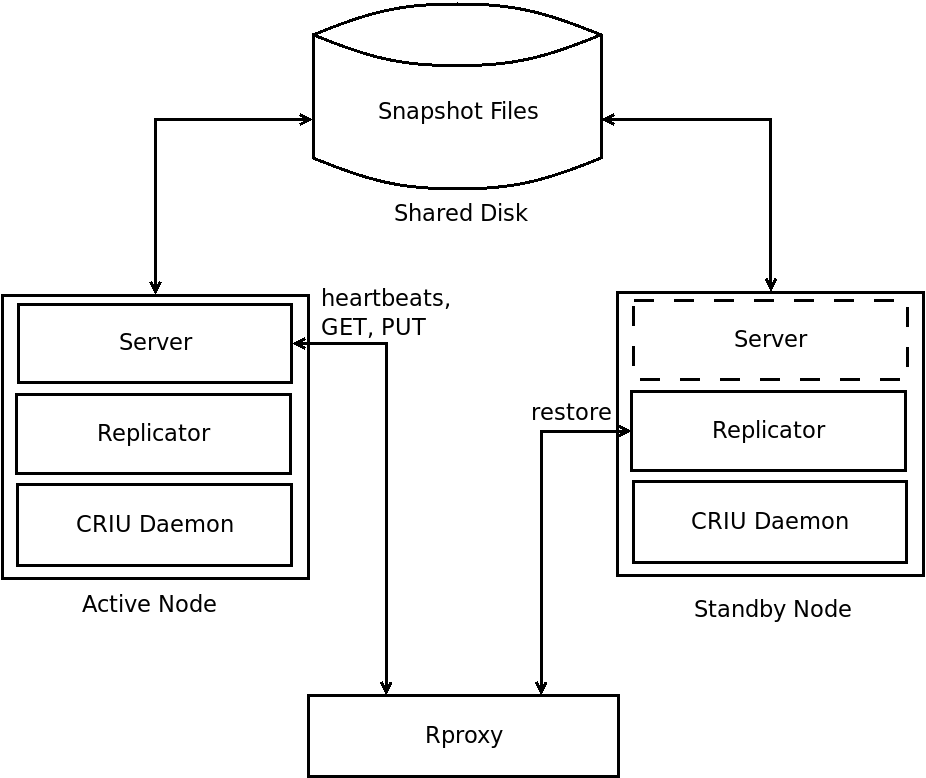
\includegraphics[width=\columnwidth]{arch}
  \caption{System Architecture.}
  \label{fig:arch}
\end{figure}

The server process is the actual key-value store that can accept and serve
requests. The implementation of the server is kept simple so we can focus on
building the replication technique. The server exposes two APIs for requests:
\verb|Put(key, value)| and \verb|Get(key)|. Note that \verb|value| here is not
an atomic type, rather, it is a set of fields that each hold a value. In our
implementation, we treat \verb|value| as a JSON object. Clients communicate with
the server over HTTP. For example, retrieving a key would involve sending a GET
request to \verb|http://server-ip/key|. Inserting a key is similar, except a PUT
request is used and the values are encoded in the request body. Internally, we
parse the request body and store the keys and their values in an in-memory hash
table. The server also keeps track of the number of PUT requests it has
received, and once a certain threshold is reached, it will notify the replicator
to capture a snapshot of itself. This is similar to how Redis RDB works, where
the user can specify a required number of writes made to the dataset after
which an RDB file will be created.

\subsubsection{Replicator}

The replicator is a thin process that acts as a wrapper around the
checkpoint/restore daemon. It exposes two APIs to control replication,
\verb|checkpoint| and \verb|restore|. The former captures a snapshot of the
server and stores it on the shared-disk, while the latter retrieves the latest
snapshot from the shared-disk and restores it. It does this by sending RPC calls
to the checkpoint/restore daemon. The \verb|checkpoint| method is called by the
server when the checkpoint interval has passed, and the \verb|restore| method is
called by the rproxy, when it detects that the server on the active node is
down.

\subsubsection{Checkpoint/Restore Daemon}

The checkpoint/restore daemon is a daemonized version of the CRIU tool. External
processes (such as the replicator) communicate with it through RPC calls over a
Unix socket. The daemon is responsible for the system-level code that
checkpoints and restores the process state of the server. A more elaborate
overview of CRIU is given in section \ref{CRIU}.

\subsubsection{Rproxy}

The rproxy is the client-facing process that is responsible for routing requests
to the active replica. On initialization, it connects to the server on the
active node and sends regular heartbeats to it. If it detects from a lapsed
heartbeat check that the server is down, it calls \verb|restore| on the
replicator of the standby node to restore the server from the latest
snapshot. Subsequently, the former standby now becomes the active replica.

\subsection{Checkpoint/Restore In Userspace}\label{CRIU}

The CRIU utility can be used to freeze the state of a running process/container
and save this state to a set of image files on persistent storage. The process
can then be restored back to the point it was frozen from the image files. It is
integrated in multiple container run-times such as OpenVZ, LXC/LXD, Docker, and
Podman. For example, Google's Borg cluster management system uses CRIU for
live-migrating jobs across their clusters \cite{marmol2018task}.

CRIU serializes the contents of a process's virtual memory address into image
files. It does so by obtaining the memory pages currently in use by the process
using the \verb|/proc| filesystem on Linux. Once it has identified the pages, it
injects parasite code into the process using \verb|ptrace| and drains the
contents of its memory into files on disk. On restore, CRIU forks itself,
applies the contents of the images files into its memory address and resumes
execution. The image files can be copied to a different machine and then
restored, making CRIU ideal for moving or replicating processes across machines.

\section{Evaluation}

\subsection{Methodology}

We use the Yahoo! Cloud Serving Benchmark (YCSB), a popular key-value store
benchmark suite for evaluating our system. It automates essential benchmarking
tasks such as workload definition, workload execution and performance
measurement. To add our key-value store to YCSB's suite, we implemented a custom
database interface layer that uses our key-value store's API. In particular, we
implemented the \verb|read|, \verb|update|, \verb|insert| and \verb|delete|
methods, omitting \verb|scan| due to time constraints. We use workloads A and B
from the YCSB suite, each of which execute 1000 operations and have a read/write
mix of 50/50 and 95/5 respectively. For replication, we configured the server to
capture snapshots after every 250 updates.


Our experiments were run on a cluster of three nodes, each with 2 Intel Xeon
E5-2620v2 processors for a total of 24 cores, and 32 GB of RAM. The active and
standby nodes are also connected to an NFS drive with 4TB of storage, which is
used as the shared-disk for storing snapshots.

\subsection{Storage Performance vs Redis}

\begin{figure}
  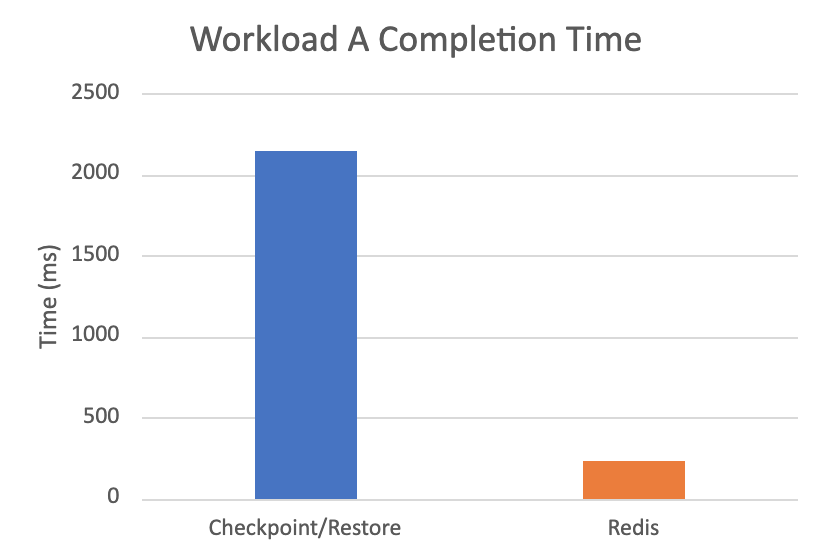
\includegraphics[width=\columnwidth]{redis-workload-A.png}
  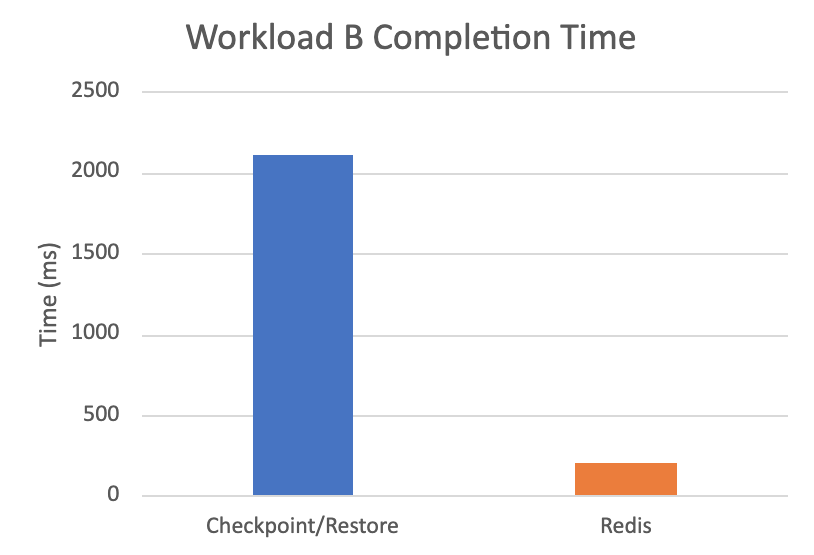
\includegraphics[width=\columnwidth]{redis-workload-B.png}

  \caption{Workload completion times for workloads A and B against Redis.}
  \label{fig:redis}
\end{figure}

To assess the baseline performance of our key-value store's storage engine, we
disabled replication and ran YCSB workloads A and B and compared it with Redis.
The results are shown in figure \ref{fig:redis}.

Note that since our focus was on the replication layer and not the storage
engine itself, we expected the performance to be subpar compared to Redis. We
believe the overhead primarily comes from using HTTP as the message protocol and
the serialization/de-serialization of JSON objects in each request.
Comparatively, Redis uses the Redis Serialization Protocol (RESP)
\cite{RedisProtocol} and an encoding scheme that is fast to parse which possibly
results in an order of magnitude better performance.

\subsection{Replication Performance vs Asynchronous Replication}

\begin{figure}
  \centering
  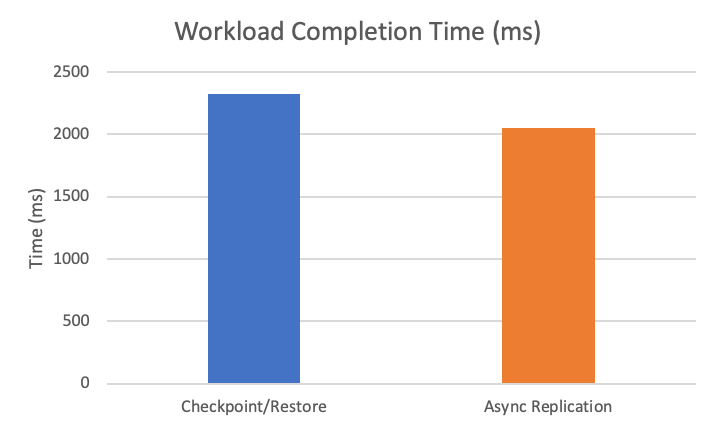
\includegraphics[width=\columnwidth]{async-replication.png}

  \caption{Workload completion times for workload A against asynchronous replication.}
  \label{fig:async-completion}
\end{figure}

We compare the performance of snapshot-based replication against asynchronous
statement-based replication. We do this by implementing the latter in our
key-value store by shipping the statement to the standby replica, after the
server has replied to the client. Note that we only use workload A for the
comparison, since workload B consists of 95\% read requests which are not enough
to trigger snapshots, causing the performance of checkpoint/restore to be the
same as asynchronous replication.

Figure \ref{fig:async-completion} shows the workload completion times by each
replication technique. Given that checkpoint/restore captures snapshots after
every 250 updates, we did expect a slight increase in completion time compared
to asynchronous replication. Recall that workload A has a 50/50 read/write mix,
which results in around 500 update operations, giving us 2 snapshots for this
run.

\begin{figure}
  \centering
  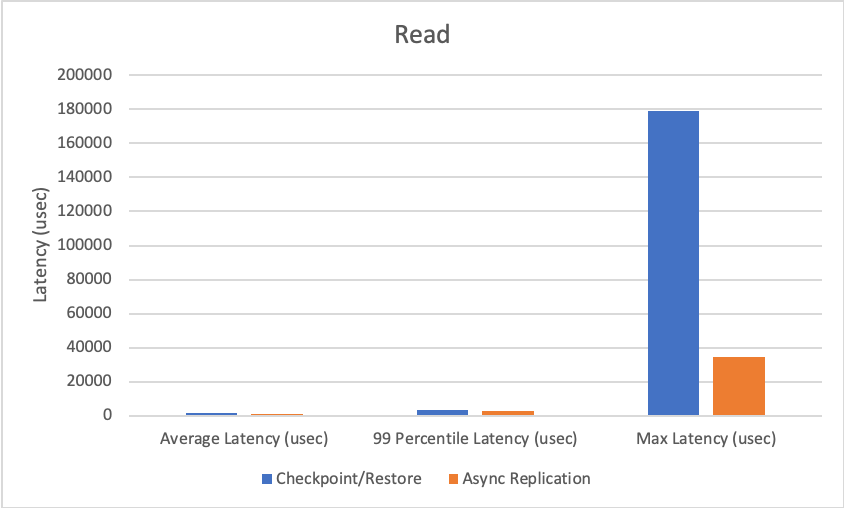
\includegraphics[width=\columnwidth]{async-replication-read.png}
  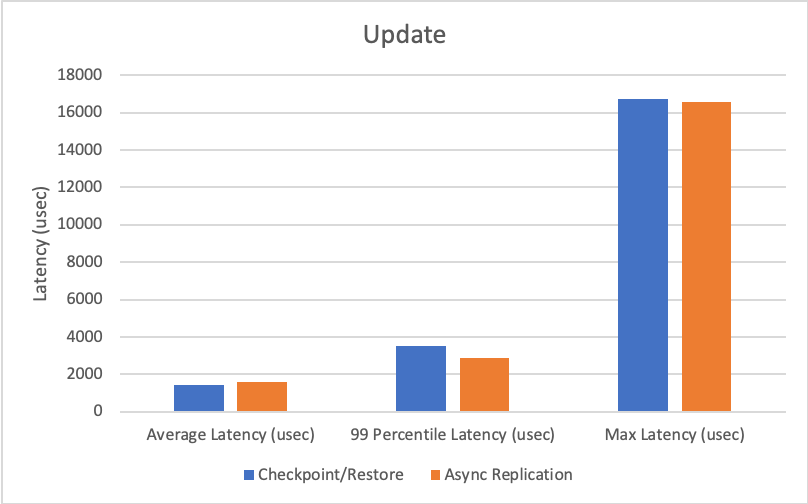
\includegraphics[width=\columnwidth]{async-replication-update.png}

  \caption{Average and max latency for read and update requests against asynchronous replication.}
  \label{fig:async-latency}
\end{figure}

Figure \ref{fig:async-latency} shows the average and max latency for read and
update requests by each replication technique. Average latencies for both types
of requests are around the same; this can be explained by the fact that the cost
of snapshotting is amortized across multiple requests. While max latencies for
update requests are the same, max latencies for read requests have a much larger
discrepancy: a wide gap exists due to unlucky read requests being blocked as a
snapshot is in progress.

\subsection{Impact of Checkpoint Intervals on Workload Completion}

\begin{figure}
  \begin{tikzpicture}[scale=0.75]
    \begin{axis}[
    xlabel=Checkpoint Intervals (\# of records),
    ylabel=Workload Completion Time (ms),
    xmin=0, xmax=2200,
    ]
    \addplot[mark=*,blue] plot coordinates {

    (250,6702)
    (500,6321)
    (750,6085)
    (1000,6082)
    (1250,5892)
    (1500,5692)
    (1750,5696)
    (2000,5681)

    };
  \end{axis}
  \end{tikzpicture}
  \caption{Checkpoint intervals vs workload completion time for a workload with 5000 insert operations.}
  \label{fig:freq}
\end{figure}

Checkpointing the state of the key-value store is an expensive operation. More
frequent checkpoints will minimize data loss due to a crash but at the cost of
performance. To assess the impact of the checkpoint interval on the performance
of the key-value store, we vary the number of writes that trigger a checkpoint
and run a custom workload consisting of 5000 insert operations. The results are
shown in figure \ref{fig:freq}. As expected, workload completion times decrease
as checkpoint intervals increase. This comes with an increase in possible data
loss, hence the exact interval will be application-dependent and can be tuned by
the user.

\subsection{Standalone vs Iterative Snapshots}

CRIU snapshots can be standalone, where the entire memory address space of the
process is checkpointed as is, or iterative, where snapshots only capture memory
pages that have changed since the last snapshot. The differences in time taken
to complete a snapshot as the dataset size increases can be seen in figure
\ref{fig:iterative}. Using standalone snapshots for frequent checkpoints would
be inefficient, since the snapshot time would be proportional to the size of the
process's memory. Iterative snapshots are more efficient, since they capture a
constant amount of data between snapshots. Our implementation uses iterative
snapshots to minimize the time that requests are blocked while a snapshot is in
progress.

\begin{figure}
  \centering
  \begin{tikzpicture}[scale=0.75]
    \begin{axis}[legend style={at={(0.35, 0.95)},anchor=north},
    xlabel=Dataset size (MB),
    ylabel=Snapshot Time (ms),
    ymin=0, ymax=600, ytick={100,200,300,400,500,600}]

    \addlegendentry{Standalone snapshots}
    \addplot[mark=*,blue] plot coordinates {
    (2,111)
    (4,126)
    (8,155)
    (16,215)
    (32,329)
    (64,498)
    };

    \addlegendentry{Iterative snapshots}
    \addplot[color=red,mark=x]
    plot coordinates {
    (2,54)
    (4,75)
    (8,84)
    (16,137)
    (32,151)
    (64,163)
    };
    \end{axis}
  \end{tikzpicture}
  \caption{Time taken for standalone vs iterative snapshots across increasing
  dataset sizes.}
  \label{fig:iterative}
\end{figure}

\section{Conclusion}

In this paper, we have explored using checkpoint/restore for replication to
guarantee HA. To that extent, we implemented a key-value store that uses
checkpoint/restore to replicate its in-memory state to another machine. Initial
results show that this approach works well with minimal overhead compared to
asynchronous statement-based replication. Further optimizations and improvements
can be made to checkpoint/restore which can result in better performance and
durability.

For example, it is possible to move from a shared-disk to a shared-nothing setup
by utilizing CRIU's page server feature. This allows the active replica to
stream image files across the network to a page server on the standby replica.

The current implementation of checkpoint/restore guarantees RDB-style
durability, which can lose data if the server crashes in between snapshots. For
stronger durability, we can implement \textit{output commit} as mentioned in
\cite{RemusDB}, where output packets are buffered until the next snapshot. This
would turn checkpoint/restore into a more synchronous replication technique,
where greater durability comes at the price of higher request latency.

Currently, the standby replica does not actually run a server process until
failover. CRIU has no existing support for applying images to a running process,
but it is a planned feature \cite{CRIUApply}. As a result, it is not viable to
convert the standby to serve read requests: new snapshots would have to kill the
running server on the standby and then restore it from the latest snapshot,
leading to frequent client disconnections. Once the apply images feature is
introduced, checkpoint/restore can be extended to have read requests be served
by the standby.

Thus, checkpoint/restore is a potentially viable replication technique with
acceptable tradeoffs between replication freedom and implementation complexity.
By delegating replication to an external layer, database systems can achieve
high availability with minimal implementation and performance overhead.

\printbibliography

\section{Appendix}

\subsection{Post-mortem}

\begin{itemize}
  \item The project was quite implementation heavy, since we had to implement
  the key-value store API, figure out the internals of CRIU and figure out how to
  run YCSB to get benchmark results.
  \item The CRIU daemon API uses gRPC and its examples were documented in Go,
  because of this, we implemented our system using Go. Since one of the authors
  has experience with Go, this was not too much of an impediment.
  \item CRIU has interesting research applications that we were eager to
  explore, but could not because of time constraints. For example, it supports
  migrating existing TCP connections from one machine to the other. This has
  some potential use-cases for live-migration scenarios.
  \item The benchmarks were run on the DSG group's tembo cluster. The /home
  directories on tembo are shared NFS drives, which made deploying our system
  easier.
  \item We initially wanted to run checkpoint/restore on top of an existing
  key-value store like Redis, but there were some issues with CRIU that made it
  difficult to checkpoint Redis, so due to time constraints we implemented a
  simple key-value store to drive our replication technique.
  \item We initially wanted to replicate at the container-level as opposed
  to the process-level, but existing container runtimes do not fully support
  some CRIU features like iterative snapshotting, so we decided to use
  CRIU at the process-level.
\end{itemize}

\end{document}
